\documentclass{article}
\usepackage[utf8]{inputenc}
\usepackage{graphicx}
\usepackage[spanish]{babel}
\usepackage{amsmath}
\usepackage{amsfonts}
\usepackage{amssymb}
\usepackage{multicol}
\usepackage{multirow}
\usepackage{bigstrut}
\usepackage{booktabs}
\usepackage{caption}
\usepackage[left=2.54cm,right=2.54cm,top=2.54cm,bottom=2.54cm]{geometry}
\spanishdecimal{.}
\begin{document}
\begin{center} \LARGE{ESCUELA POLITECNICA NACIONAL} \\[0.5cm] \Large{FACULTAD DE INGENIERÍA EN SISTEMAS}\\[0.5cm] \large{PROBABILIDAD Y ESTADISTICA} \end{center}
\begin{figure}[htb] \centering 
\includegraphics[scale=.6]{descarga (1).png}\end{figure}
\begin{center} \large{\bf Proyecto 2° Bimestre:}\\ \vspace{.25cm} { \Large \bfseries \underline{UN CLIMA SABOR A CAFÉ}} \\ \end{center}
\large{\bf Estudiantes: Rafael Alexander Piedra Granda, Christofer Alexander Villamarín Pila, Darwin Guachamin  }\\
\large{\bf Docente: Monica Mantilla }\\
\large{\bf Grupo: }\\\begin{center} \Large \textsc{Quito - Ecuador} \\
\Large \textsc{2022}
\end{center}
\pagebreak
\section{Introduccion}
El presente trabajo tiene como finalidad conseguir la sostenibilidad del emprendimiento mediante el análisis e interpretación de los datos recolectados en un periodo de tiempo, el cual consiste en un cibercafé administrado por estudiantes de la facultad de ciencias administrativas de la universidad estatal de Indiana, Estados Unidos . Anteriormente debido a la falta de un rigor estadístico, muchos emprendimientos de alimentación dentro de la facultad fracasaron, sin embargo con métricas claras se reduce la complejidad de tomar decisiones financieras. Mediante el uso de la estadística inferencial es posible determinar mediante una pequeña porción de los datos la tendencia general de la población, permitiendo así interpretaciones más rápidas de los resultados y agilizando la toma de decisiones. Una vez se normalice el continuo análisis e interpretación de la información de la  base de datos, se obtendrá una manera de proyectar la tendencia general de los datos hacia futuras expansiones del negocio,generando un modelo de negocio escalable a largo plazo. La interpretación de los datos es de suma importancia para que los negocios cuenten con un respaldo en la toma de sus decisiones. 
\section{Metodologia}
Los datos utilizados para el estudio fueron recolectados de un café dirigido por estudiantes de negocios en una universidad pública de Estados Unidos. Los datos se recopilaron durante un período de diez semanas durante el semestre de primavera de 2010.\\\\
Para la maquetación de proyecto de hizo uso de la herramienta latex:\\
\begin{center}
    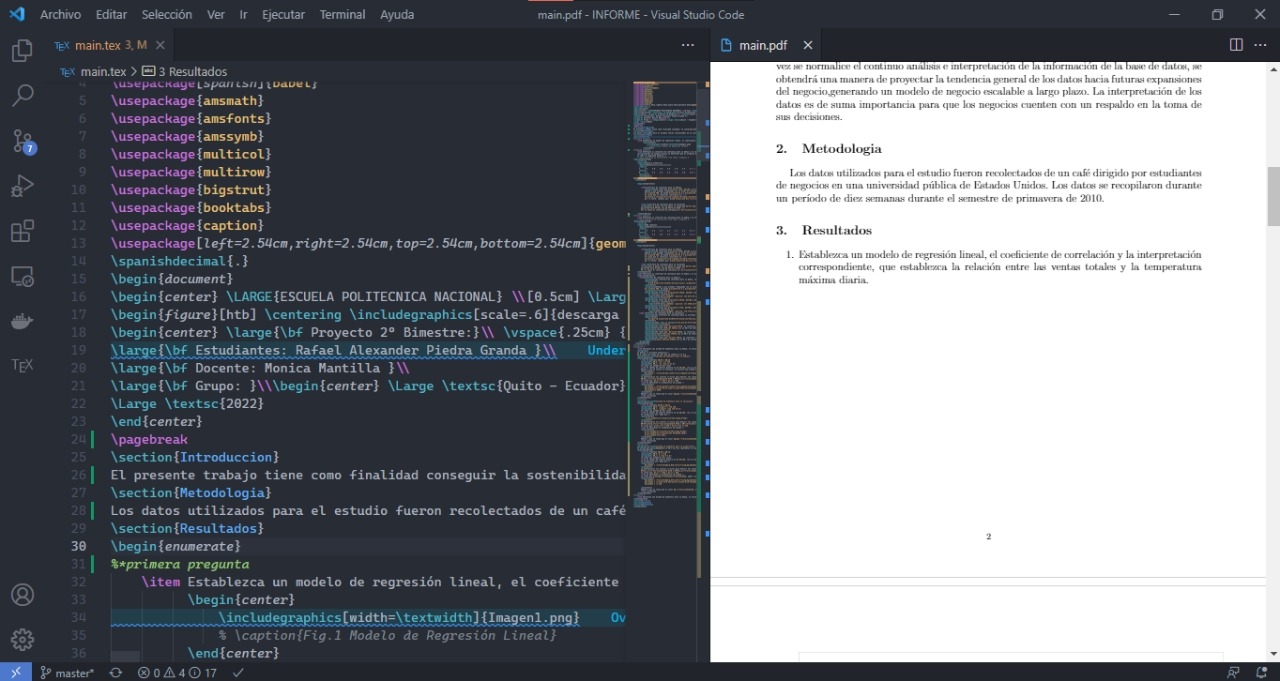
\includegraphics[width=\textwidth]{WhatsApp Image 2022-02-28 at 1.07.56 AM.jpeg}
    
\end{center}
\section{Resultados}
\begin{enumerate}
%*primera pregunta  
    \item Establezca un modelo de regresión lineal, el coeficiente de correlación y la interpretación correspondiente, que establezca la relación entre las ventas totales y la temperatura máxima diaria.
          \begin{center}
              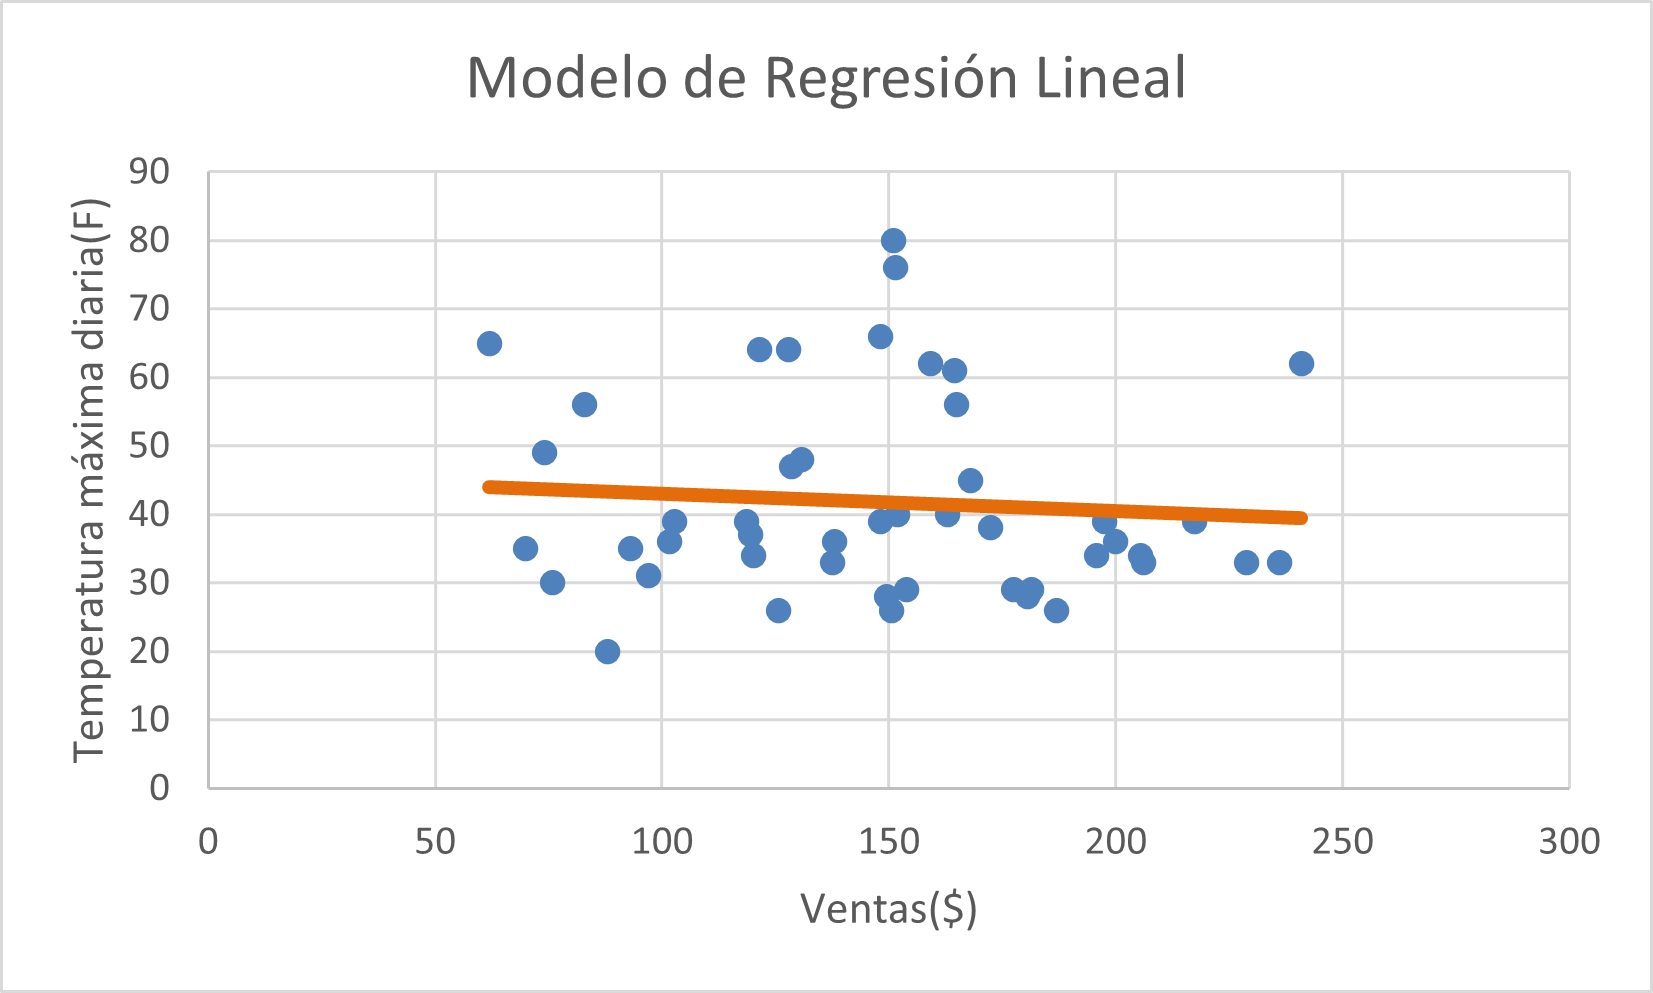
\includegraphics[width=\textwidth]{Imagen1.png}
              
          \end{center}
%*segunda pregunta  
    \item Determine un intervalo de confianza para la media y la varianza para el producto que más se desperdicia, con un nivel de confianza del 98%.
    \paragraph{}En un estudio previo se determinó que el producto que mas se vendió fueron los wraps, a continuación se determinan los intervalos de confianza para el producto.
    se tomó la siguiente muestra:\\
    % Table generated by Excel2LaTeX from sheet 'pregunta 2'
\begin{table}[htbp]
    \centering
    \caption{muestra aleatoria}
      \begin{tabular}{|c|c|c|c|c|c|c|c|}
      \toprule
      1     & 3     & 0     & 0     & 0     & 0     & 3     & 7 \\
      \midrule
      0     & 5     & 4     & 9     & 2     & 0     & 0     & 0 \\
      \bottomrule
      \end{tabular}%
    \label{tab:addlabel}%
  \end{table}%
   
    \begin{enumerate}{}
       
        \item{intervalo de confianza para la media}
            \paragraph{}Se tiene que $\bar{x}=2.125$, $n=16$ y $\sigma=7.61$.\\
            Debido a que estamos trabajando con un nivel de confianza del 98\%, por lo tanto se tiene que:\\ 
            $1-\alpha=0.98$, de donde $\alpha=0.02 $ y $\alpha/2=0.01$, por lo tanto, $z_{0.01}=2.33$ 
            Se tiene que el intervalo resultante es: \\\\
            $(\bar{x}-z_{\alpha/2}\frac{\sigma}{\sqrt{n}};\bar{x}+z_{\alpha/2}\frac{\sigma}{\sqrt{n}})=(3.73,21.83)$\\\\
            por lo tanto, tenemos que: $\mu$ $\epsilon$ $(3.73,21.83)$ con un 98\% de confianza
        

        \item {intervalo de confianza para la varianza}
        \paragraph{} A partir de los datos se tiene que $s^2=7.61$,$n=16$ y $1-\alpha=0.98$, ademas a partir de la tabla de la distribución chi-cuadrado con 15 grados de libertad se tiene que: \\\\
        $x_{0.01}^2=30.5779$ y $x_{0.99}^2=5.2294$ \\\\
        Por lo tanto el intervalo de confianza es: $(\frac{(n-1)s^2}{x_{\alpha/2}^2(n-1)};\frac{(n-1)s^2}{x_{1-\alpha/2}^2(n-1)})=(3.73;21.83)$ 
        
    \end{enumerate}
%*tercera pregunta    
    \item Determine un intervalo de confianza para la media y la varianza para la copa de frutas, con un nivel de confianza del 98%.
    % Table generated by Excel2LaTeX from sheet 'pregunta 3'
\begin{table}[htbp]
    \centering
    \caption{Add caption}
      \begin{tabular}{|c|c|c|c|c|c|c|c|}
      \toprule
      1     & 4     & 3     & 2     & 1     & 2     & 2     & 2 \\
      \midrule
      2     & 4     & 2     & 0     & 2     & 1     & 0     & 2 \\
      \bottomrule
      \end{tabular}%
    \label{tab:addlabel}%
  \end{table}%
  
    \begin{enumerate}{}
       
        \item{intervalo de confianza para la media}
            \paragraph{}Se tiene que $\bar{x}=1.875$, $n=16$ y $\sigma=1.15$.\\
            Debido a que estamos trabajando con un nivel de confianza del 98\%, por lo tanto se tiene que:\\ 
            $1-\alpha=0.98$, de donde $\alpha=0.02 $ y $\alpha/2=0.01$, por lo tanto, $z_{0.01}=2.33$ 
            Se tiene que el intervalo resultante es: \\\\
            $(\bar{x}-z_{\alpha/2}\frac{\sigma}{\sqrt{n}};\bar{x}+z_{\alpha/2}\frac{\sigma}{\sqrt{n}})=(1.21,2.54)$\\\\
            por lo tanto, tenemos que: $\mu$ $\epsilon$ $(1.21,2.54)$ con un 98\% de confianza
        
        \item {intervalo de confianza para la varianza}
        \paragraph{} A partir de los datos se tiene que $s^2=1.23$,$n=16$ y $1-\alpha=0.98$, ademas a partir de la tabla de la distribución chi-cuadrado con 15 grados de libertad se tiene que: \\\\
        $x_{0.01}^2=30.5779$ y $x_{0.99}^2=5.2294$ \\\\
        Por lo tanto el intervalo de confianza es: $(\frac{(n-1)s^2}{x_{\alpha/2}^2(n-1)};\frac{(n-1)s^2}{x_{1-\alpha/2}^2(n-1)})=(0.60;3.53)$ 
    \end{enumerate}
    \item Determine un intervalo de confianza para la media y la varianza para los tres productos más vendidos, con un nivel de confianza del 98\%.
    \begin{enumerate}{}
      \item{Intervalo de confianza para la media:}
			\paragraph{}El intervalo de confianza para la media, con varianza muestral se define:
      	  	\begin{center}
      	  		$\mu$ $\epsilon$ $\left(\bar{x}-t_{(n-1,\alpha/2)}\dfrac{s}{\sqrt{n}};\bar{x}+t_{(n-1,\alpha/2)}\dfrac{s}{\sqrt{n}}\right)$
			\end{center} 		     	  	 
      	  	\paragraph{}Debido a que estamos trabajando con un nivel de confianza del 98\% y n=48, se obtiene: 
          	$1-\alpha=0.98$, de donde $\alpha=0.02 $ y $\alpha/2=0.01$, por lo tanto $t_{(47,0.01)}=2.4083$.
          	\paragraph*{}\textbf{Sodas}
          	\paragraph{}Se tiene que $\bar{x}=28.9583$, $n=48$ y $s=12.4882$.
          		El intervalo resultante es:
          		\begin{center}$\mu_{sodas}\ \epsilon\ (24.6172,33.2993)$ con un 98\% de confianza.\end{center}
          	\paragraph*{}\textbf{Cafés}
          	\paragraph{}Se tiene que $\bar{x}=21.0625$, $n=48$ y $s=11.3932$.
          		El intervalo resultante es:
          		\begin{center}$\mu_{cafes}\ \epsilon\ (17.1020,25.0229)$ con un 98\% de confianza.\end{center}
          	\paragraph*{}\textbf{Wraps}
          	\paragraph{}Se tiene que $\bar{x}=12.875$, $n=48$ y $s=6.1076$.
          		El intervalo resultante es:
          		\begin{center}$\mu_{wraps}\ \epsilon\ (10.7743,15.0206)$ con un 98\% de confianza.\end{center}
      \item {Intervalo de confianza para la varianza:}
			\paragraph{}El intervalo de confianza para la varianza se define como:
			\begin{center}
				$\sigma^2$ $\epsilon$ $\left(\dfrac{(n-1)s^2}{\chi_{(\alpha/2,n-1)}^2};\dfrac{(n-1)s^2}{\chi_{(1-\alpha/2,n-1)}^2}\right)$
			\end{center}	
			\paragraph{}Aquí solo se calcula $\chi_{(0.01,47)}^2=27.4158$ y $\chi_{(0.99,47)}^2=72.4433$          	
          	\paragraph*{}\textbf{Sodas}
			\paragraph{}Se tiene que: $s^2=155.9557$. El intervalo resultante es:
			\begin{center}$(101.1810;267.3601)$ con un 98\% de confianza.\end{center}			
          	\paragraph*{}\textbf{Cafés}
  			\paragraph{}Se tiene que: $s^2=129.8045$. El intervalo resultante es:      	
			\begin{center}$(84.2153;222.5299)$ con un 98\% de confianza.\end{center}          
          	\paragraph*{}\textbf{Wraps}
			\paragraph{}Se tiene que: $s^2=37.3031$. El intervalo resultante es:   	
			\begin{center}$(24.2014;63.9496)$ con un 98\% de confianza.\end{center}
      \paragraph{}
  \end{enumerate}
%!preguntas 5 y 6 
%*pregunta 5
    \item Determine una prueba de hipótesis para la media, la varianza y la proporción para el número de tazas de café que se venden por día, con un nivel de confianza del 98%.
    \paragraph{}
    se define la variable aleatoria:\\
    $x:$ numero de tazas de café que se venden en un día 
    \paragraph*{}\textbf{prueba de hipótesis para la media}\\
    \begin{enumerate}
        \item se plantean $H_0$ y $H_1$
        \paragraph{} $H_0: \mu = 21.51$
        \paragraph{} $H_1: \mu \neq 21.51 $\\
        se tiene una prueba de dos colas 
        \item El tamaño de nuestra muestra es de $n=16$, con un nivel de significancia del 5\%, en consecuencia $\alpha = 0.05$ y $\alpha/2 =0.025$.\\
        Debido a que se conoce la varianza, se utilizó una prueba $Z$ cuyo estadistico está dado por:\\
        \begin{center}
            $Z_{stat} = \frac{\bar{x}-\mu}{\frac{\sigma}{\sqrt{n}}}$\\
        \end{center}
        se determinaron los valores críticos para definir las zonas de rechazo y no rechazo, por ello se tiene que: \\
        $P(Z<z_1)=\frac{\alpha}{2}=0.025$ y $P(Z>z_2)=\frac{\alpha}{2}=0.025$\\
        se tiene que: $z_1= -1.96$ y $z_2= 1.96$
        \item Se determinó el estadistico de prueba \\
        \begin{center}
            $Z_{stat} = \frac{\bar{x}-\mu}{\frac{\sigma}{\sqrt{n}}}$\\ 
            $Z_{stat}=\frac{18.69-21.51}{\frac{10.96}{\sqrt{16}}}$\\             
            $Z_{stat}=-1.029$
        \end{center}
        Debido a que se tiene que el valor $p\geq \frac{\alpha}{2}$, es decir $P(Z>1.96)\geq 0.25$, dado que $P(Z>1.96)=0.025$, la hipótesis no se rechaza 
        \item conclusion
    \end{enumerate}
    %*varianza
    \paragraph*{}\textbf{prueba de hipótesis para la varianza}\\
    \begin{enumerate}
        \item se plantean $H_0$ y $H_1$
        \paragraph{} $H_0: \sigma^2 = 120.16$
        \paragraph{} $H_1: \sigma^2 \neq 120.16 $\\
        se tiene una prueba de dos colas 
        \item El tamaño de nuestra muestra es de $n=16$, con un nivel de significancia del 5\%, en consecuencia $\alpha = 0.05$ y $\alpha/2 =0.025$.\\
        El estadistico está dado por:\\
        \begin{center}
             $\chi_{stat}^2=\frac{(n-1)s^2}{\sigma_0^2}$\\
        \end{center}
        se determinaron los valores críticos para definir las zonas de rechazo y no rechazo, por ello se tiene que: \\
        $P(X^2(15)<X_1^2)=\frac{\alpha}{2}=0.025$ y $P(\chi^2(15)>\chi_2^2)=\frac{\alpha}{2}=0.025$\\
        se tiene que: $\chi_1^2= 6.26$ y $\chi_2^2= 27.35$
        \item Se determinó el estadistico de prueba \\
        \begin{center}
            $\chi_{stat}^2=\frac{(n-1)s^2}{\sigma_0^2}$\\
            $\chi_{stat}^2=\frac{(15)(107.44)}{120.10}$\\
            $\chi_{stat}^2=13.42$\\
        \end{center}
        Debido a que se tiene que el valor $p\geq \frac{\alpha}{2}$, es decir $P(X^2>27.35)\geq 0.25$, dado que $P(X^2>27.36)=0.026$, la hipótesis no se rechaza 
        \item conclusion
    \end{enumerate}
    %*proporción
    \paragraph*{}\textbf{prueba de hipótesis para la proporción}\\
    Se estima que aproximadamente el 60\% de días laborables se vendieron más de 30 tazas de café. Se tomó una muestra aleatoria en la cuál se venden más de 30 tazas de café.   
    \begin{enumerate}
        \item se plantean $H_0$ y $H_1$
        \paragraph{} $H_0: p = 0.6$
        \paragraph{} $H_1: p \neq 0.6 $\\
        se tiene una prueba de dos colas 
        \item El tamaño de nuestra muestra es de $n=16$, con un nivel de significancia del 5\%, en consecuencia $\alpha = 0.05$ y $\alpha/2 =0.025$.\\
        El estadistico está dado por:\\
        \begin{center}
            $Z_{stat} = \frac{\hat{p}-p_0}{\sqrt{\frac{p_0q_0}{n}}}$\\ 
        \end{center}
        se determinaron los valores críticos para definir las zonas de rechazo y no rechazo, por ello se tiene que: \\
        $P(Z<z_1)=\frac{\alpha}{2}=0.025$ y $P(Z>z_2)=\frac{\alpha}{2}=0.025$\\
        se tiene que: $z_1= -1.96$ y $z_2= 1.96$
        \item Se determinó el estadistico de prueba \\
        se tiene que $\hat{p}=\frac{x}{n}=\frac{11}{48}$, además sabemos que $q_{0}=1-p_{0}$, por lo tanto $q_{0}=0.5$
        \begin{center}
            $Z_{stat} = \frac{\hat{p}-p_0}{\sqrt{\frac{p_0q_0}{n}}}$\\ 
            $Z_{stat} = \frac{0.23-0.5}{\sqrt{\frac{(0.5)(0.5)}{16}}}$\\
            $Z_{stat} = -2.16$

        \end{center}
        Debido a que se tiene que el valor $p <\frac{\alpha}{2}$, es decir $P(Z>1.96)< 0.25$, dado que $P(Z>)=0.026$, la hipótesis no se rechaza 
        \item conclusion
    \end{enumerate}
%*pregunta 6
    \item Determine una prueba de hipótesis para la media, la varianza y la proporción para el total de ventas, con un nivel de confianza del 98%
\end{enumerate}
\section{Análisis}
\section{Apéndices}
\section{Referencias}
\end{document}